% !TEX root = main.tex
% Target, model, credit and optimization; conditional readout convergence.
\begin{abstract}
Step supervision can train a Transformer that fails to learn from final answers alone.
We explain this gap through gradient credit. A target splits into interactions among input
moves. Each interaction receives credit only from the matching part of the model's Jacobian.
In permutation tasks, every unseen move contracts this credit. Long answers therefore give
little signal to a fresh Transformer, whose Jacobian is mostly low-degree.
For a two-block Transformer at small initialization, we bound outcome interaction credit
and prove a near-chance plateau of duration $\Omega(\min(\initscale^{-2},\mixrate^{-n}))$.
Step targets retain credit for the transition rule without exponential decay in $n$.
From a zero-readout start, outcome training does not reach an exact solution for time
$\Omega(\mixrate^{-n})$; step training converges to an exact solution once its loss falls below an
explicit threshold. Whether step training reaches that threshold remains open.
In counting over $16$ letters, step training solves nine of ten seeds; outcome training stays
at chance on nine. On three-object BIG-Bench Hard tracking, LoRA-tuned Qwen2.5-0.5B reaches
$98$--$100\%$ with steps and stays at the majority-option rate with answers alone.
\end{abstract}

\section{Introduction}
\label{sec:intro}

Consider counting a query letter modulo $3$ (\cref{tab:rows}). We can train on the final
count alone, or on the running counts as well. We call these \emph{outcome} and \emph{step}
supervision. With matched initialization, data and training budget, outcome training stays
at chance while step training solves the task (\cref{tab:main}). The same two-block
architecture can execute either format exactly (\cref{prop:represent}). Why does training
find one solution more readily?

The answer is a mismatch between the target and the features available at initialization.
For a two-letter word, the answer splits into a constant, a piece for each letter, and a
piece that depends on both letters. A feature of the first letter receives credit only from
the first-letter piece. As the word grows, this piece shrinks geometrically.
Most of the answer then lies in interactions among many letters.

We call the number of moves in an interaction its \emph{degree}.
A fresh Transformer has little sensitivity to high-degree interactions.
Long outcome targets therefore provide little usable credit.
A step target depends on the displayed state and one move. It avoids the long unseen
horizon (\cref{fig:credit}).

\begin{figure}[t]
\centering
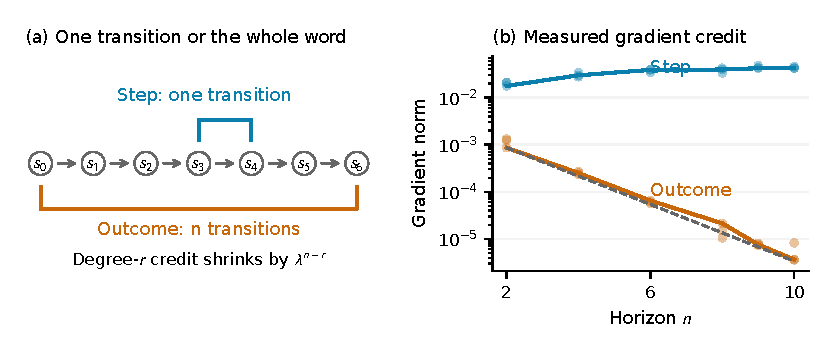
\includegraphics[width=\linewidth]{figures/credit_locality.pdf}
\caption{\textbf{The answer touches $n$ transitions, a step target only one.} (a)~A degree-$r$
feature of the answer is damped by $\mixrate^{n-r}$, and a step target shortens the horizon to $1$.
(b)~Measured on a two-block Transformer at initialization, the answer gradient decays at the
predicted rate $\mixrate=0.5$ per letter and the step gradient does not
(\cref{tab:spectrum}).}
\label{fig:credit}
\end{figure}

\paragraph{Results.} Let $n$ be the horizon, $\initscale$ the initialization scale, and
$\mixrate<1$ the contraction per unseen move. We answer three questions.
\begin{itemize}[leftmargin=*,itemsep=3pt,topsep=3pt]
\item \textbf{Does a solution exist? Yes: exact two-block executors for both formats (\cref{prop:represent}).}
\item \textbf{How does training start? With a credit gap (\cref{thm:main,thm:separation}).}
Outcome interaction credit is at most $C\initscale^6\mixrate^{n-3}$. For counting with a fixed query,
step rule credit is of order $\initscale^6/n$ with high probability, with no factor $\mixrate^n$.
\item \textbf{Is a solution reached? Not by outcome training (\cref{thm:outcome-end}); by step
training once its loss is small (\cref{thm:basin}).} From a zero readout, outcome training stays near
chance and reaches no exact solution for time $\Omega(\mixrate^{-n})$. Step training whose loss falls
below $\pimin/4$ converges to an exact solution, and greedy decoding is then exact (\cref{cor:exact}).
\end{itemize}
Whether step training from initialization reaches that loss remains open. Experiments test whether
joint training does, and test the credit mechanism in deeper and pretrained models.

\paragraph{Scope.} The credit theorems use two blocks, fixed widths, small initialization,
full-batch gradient descent and a fixed ReLU pattern, without LayerNorm.
Target contraction applies to permutation tasks, including non-commuting moves.
A strong horizon penalty requires $\mixrate$ bounded away from $1$.
The counting executors use widths that grow with $n$, separately from the fixed-width training bounds.

Weak gradients for composed targets are known \citep{shalevshwartz2017failures}.
Our contribution is to resolve credit by interaction degree for both a fixed target and
the Transformer Jacobian. This identifies the signal that disappears and the features
that could receive it.

\begin{table}[t]
\centering\small
\begin{tabular*}{\linewidth}{@{\extracolsep{\fill}}lll@{}}
\toprule
Format & Row ($K=3$, start $1$, query \texttt a, word \texttt{banana}) & Loss on\\
\midrule
Outcome & \texttt{1 a b a n a n a SEP : 1 EOS} & ${:}\ \ 1\ \ \textsc{eos}$\\
Step & \texttt{1 a b a n a n a SEP 1 2 2 0 0 1 : 1 EOS} & \texttt{1 2 2 0 0 1} ${:}\ \ 1\ \ \textsc{eos}$\\
\bottomrule
\end{tabular*}
\caption{\textbf{The running example.} Count the letter \texttt a in \texttt{banana} modulo $3$,
starting from $1$. Both formats receive the same prompt; step supervision also generates the
running values.}
\label{tab:rows}
\end{table}

\section{Setup}
\label{sec:setting}

\begin{definition}[State-tracking task]
\label{def:task}
A task has $K$ states, a start state $s_0$, a query $q$ and moves $x_1,\ldots,x_n$, which determine
\begin{equation}
 s_t=F(s_{t-1},x_t),\qquad t=1,\ldots,n.
 \label{eq:tracking}
\end{equation}
The answer is $y=s_n$. Given $q$, the moves are i.i.d.\ and independent of $s_0$. The task is a
\emph{permutation task} if every move $x$ permutes the states; $\bm T_x$ is its permutation matrix,
so $\bm e_{s_t}^\top=\bm e_{s_{t-1}}^\top\bm T_{x_t}$.
\end{definition}
For counting, $x_t=\mathbf 1[w_t=q]$ for the $t$-th letter $w_t$, and $F(s,x)=s+x\bmod K$.

\begin{definition}[Contraction coefficient]
\label{def:lambda}
For a permutation task, let $\overline{\bm T}=\E_x\bm T_x$ and
$\mixrate=\max_q\max_{\bm v\perp\one,\|\bm v\|=1}\|\bm v^\top\overline{\bm T}\|$.
\end{definition}
Always $\mixrate\le1$: one unseen move shrinks the centred state by at most a factor $\mixrate$.
For counting over four uniform letters, $\mixrate=0.5$ at $K=2$ and $0.66$ at $K=3$
(\cref{tab:family} gives the other tasks).

\begin{definition}[Outcome and step losses]
\label{def:losses}
Let $\bm z_t(\theta)\in\R^K$ be the state logits at the position that predicts $s_t$, and $\bm z_\theta$
those at the answer position. The \emph{outcome loss} is $\Lout(\theta)=\E[-\log\softmax(\bm z_\theta)_y]$.
The \emph{step loss} is the teacher-forced loss
$\Lstep(\theta)=\frac1n\sum_{t=1}^n\E[-\log\softmax(\bm z_t(\theta))_{s_t}]$; $\Lstep^{\ge2}$ averages
over $t=2,\ldots,n$ only.
\end{definition}

Fix the start state and the query, so the moves are independent. Every square-integrable function
$f$ of the moves has a unique Efron--Stein decomposition $f=\sum_{S\subseteq[n]}f_S$, where $f_S$
depends only on $x_S$ and has mean zero in each $x_t$, $t\in S$ \citep{efron1981jackknife}.

\begin{definition}[Degree]
\label{def:degree}
The component $f_S$ has \emph{degree} $|S|$, and $(f)_r=\sum_{|S|=r}f_S$. Vector- and
matrix-valued functions are decomposed entrywise.
\end{definition}
For centred moves, $x_1+x_2$ has degree $1$ and $x_1x_2$ has degree $2$. Degree counts input
moves, not powers of parameters.

\begin{assumption}[Architecture]
\label{ass:arch}
A causal Transformer with two blocks of softmax heads and ReLU MLPs, learned token and position
embeddings, no LayerNorm, fixed widths and a linear readout $V$; every logit vector is $\bm z=Vh$ with
$h$ independent of $V$.
\end{assumption}

\begin{assumption}[Initialization]
\label{ass:init}
$\theta_0=\initscale\tilde\theta$, where $\tilde\theta$ has MLP biases $|\tilde b_m|\ge1$ and value-token
embeddings with smallest singular value $\varsigma>0$. We work on
$\initball=\{\theta:\|\theta-\theta_0\|\le\ballradius\initscale\}$ with $\ballradius=\min(1/8,\varsigma/4)$.
\end{assumption}

\begin{assumption}[Task]
\label{ass:task}
The task is a permutation task with contraction $\mixrate<1$.
\end{assumption}

\begin{assumption}[Training]
\label{ass:gd}
Full-batch gradient descent $\theta_{j+1}=\theta_j-\stepsize\nabla L(\theta_j)$ on $\Lout$ or $\Lstep$.
\end{assumption}

On $\initball$, for $\initscale$ below a constant, no ReLU unit changes sign on any input
(\cref{app:network}). Constants $c,C>0$ depend only on the widths, $K$ and $\tilde\theta$, never on
$n$, $\initscale$ or $\stepsize$ (details in \cref{app:assumptions}).

\paragraph{Target spectrum.} On a permutation task, every unseen move contracts the centred state. For every set $S$,
\begin{equation}
 \mathbb E\bigl\|(y-\bm u)_S\bigr\|^2\le\Bigl(1-\frac1K\Bigr)\mixrate^{2(n-|S|)},
 \label{eq:horizon}
\end{equation}
A component on $r$ moves averages over the other $n-r$ moves.
Each unseen move contributes one factor $\mixrate$.
Counting attains the exponent (\cref{rem:tight}).
For $\mixrate$ close to $1$, the bound can be weak at short horizons.
We also measure the target spectrum directly.


\section{Both solutions exist}
\label{sec:executors}

For counting, the same architecture can solve both formats.

\begin{proposition}[Both solutions exist]
\label{prop:represent}
For every $K$, alphabet size and $n$, there is one architecture as in \cref{ass:arch}, with widths
growing linearly in $n$, and parameters $\thstep$ and $\thout$ at which greedy
decoding produces the correct step continuation and the correct outcome continuation, respectively,
on every counting prompt. Both have a positive logit margin on every supervised position and are
exact on an open neighbourhood.
\end{proposition}

\paragraph{Construction.} Block~1 copies the query to each letter and computes its match bit
$b_t=\mathbf 1[w_t=q]$. In the step executor, Block~2 reads $s_{t-1}$ and $b_t$, then looks up
$(s_{t-1}+b_t)\bmod K$. In the outcome executor, it averages the bits, rescales by $n$, and
looks up $(s_0+\sum_t b_t)\bmod K$ (\cref{fig:executors}).
Unused heads and MLP units are zero, so both use the same architecture.
Finite routing scores keep attention leakage below the readout margin.
The positive margin and continuity give the open neighbourhood at each fixed $n$.
\Cref{app:architectures} gives the parameters and proof.
This follows the approach of explicit Transformer constructions
\citep{akyurek2023icl,ramesh2023capable}.

\begin{figure}[t]
\centering
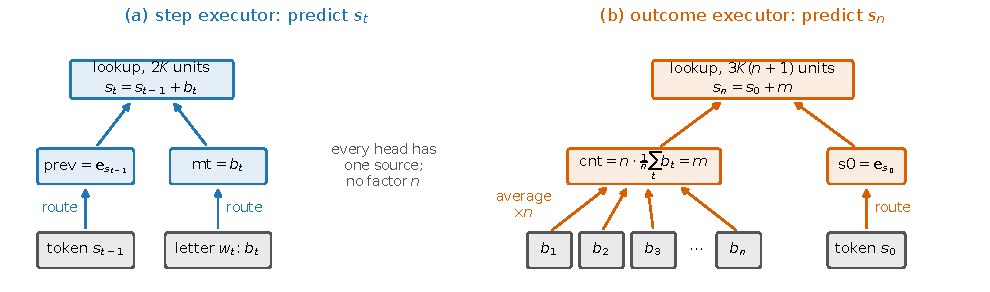
\includegraphics[width=\linewidth]{figures/executors.pdf}
\caption{\textbf{The two executors differ only in their second block.} (a)~The step executor
routes the displayed state and the current bit to a lookup with $2K$ units. (b)~The outcome
executor averages all $n$ bits, multiplies the average by $n$, and looks up $(s_0,m)$ with
$3K(n+1)$ units.}
\label{fig:executors}
\end{figure}


\section{How training starts: a credit gap}
\label{sec:gap}

\paragraph{Model spectrum at initialization.}
At small initialization, attention is nearly uniform and the MLPs are affine on $\initball$.
Uniform attention makes the network additive across positions, with degree at most $1$.
A term with $k\ge1$ attention scores reaches at most $2k+1$ input moves and has Jacobian of size
$C\initscale^2(\attconst\initscale^4)^k$: the first score permits interactions at cost $\initscale^6$, and each
further score costs $\initscale^4$ (\cref{prop:score-degree}).

\subsection{Credit matches degree}
\label{sec:credit}

\begin{definition}[Credit]
\label{def:credit}
For a target signal $g$, a random vector in $\R^K$, let $\cred_g(\theta)=\E\langle\bm z_\theta,g\rangle$.
The \emph{credit} for $g$ is $\|\nabla_\theta\cred_g(\theta)\|$, and the \emph{credit at degrees} $R$ is
$\bigl\|\sum_{r\in R}\E[(\Jz)_r^\top(g)_r]\bigr\|$.
\end{definition}
For the outcome signal $g_{\mathrm{out}}=y-\bm u$, credit is the target-dependent part of the gradient of
$\Lout$ \citep{shalevshwartz2017failures,abbe2025parities}; write $\outcredit=\cred_{g_{\mathrm{out}}}$.
The \emph{interaction credit} is the credit at degrees $r\ge2$.

Represent the answer $y$ as a one-hot vector.
Let $\bm z_\theta$ be the logits, $\hat y=\softmax(\bm z_\theta)$ and $\bm u=\one/K$.
For one prompt, $-\pd{\ell}{\theta}=(\Jz)^\top(y-\hat y)$.
Interactions on different sets of moves are orthogonal.
At uniform prediction, this gives

\begin{equation}
 -\dpd{\Lout}{\theta}
 =\sum_{r=0}^n
 \mathbb E\biggl[
 \Bigl(\dpd{\bm z_\theta}{\theta}\Bigr)_r^{\!\top}
 (y-\bm u)_r
 \biggr].
 \label{eq:grad-split}
\end{equation}
Only matching degrees contribute.
Away from uniform prediction, the same identity holds for the answer-dependent gradient
(\cref{lem:gradient-split}). Define the target and Jacobian spectra by

\begin{equation}
 A_r:=\mathbb E\bigl\|(y-\bm u)_r\bigr\|^2,
 \qquad
 J_r(\theta):=\mathbb E\bigl\|(\Jz)_r\bigr\|_F^2.
 \label{eq:spectra}
\end{equation}
Cauchy--Schwarz gives
\[
 \boxed{\text{degree-$r$ credit}\le\sqrt{A_rJ_r}}.
\]
Credit is small wherever either spectrum has little mass.

\subsection{Why outcome optimization stalls}
\label{sec:spectrum}

\begin{figure}[t]
\centering
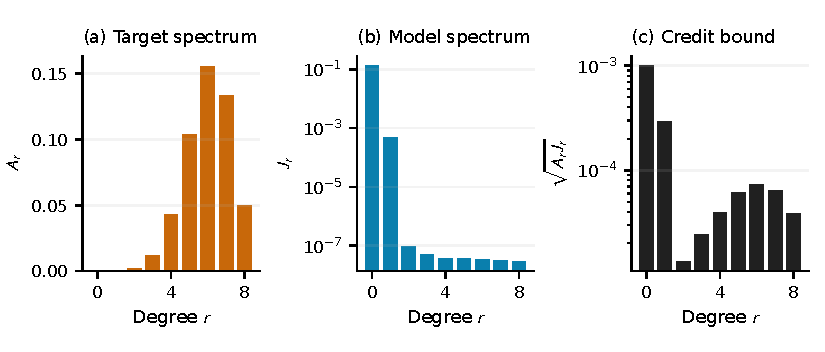
\includegraphics[width=\linewidth]{figures/overlap_spectra.pdf}
\caption{\textbf{The answer and a fresh network barely overlap.} Counting, $K=2$, $n=8$.
(a)~The target spectrum $A_r$ puts its mass at high degree. (b)~The Jacobian spectrum $J_r$ of the
two-block Transformer at initialization is $99.6\%$ degree~$0$. (c)~The bound $\sqrt{A_rJ_r}$ on the
degree-$r$ credit.}
\label{fig:overlap}
\end{figure}

\paragraph{Outcome credit and the plateau.}
\label{sec:main}

\begin{theorem}[Outcome interaction credit]
\label{thm:main}
Suppose \cref{ass:arch,ass:init,ass:task} hold, and fix the start state and the query. For all
$n\ge2$, all $\initscale$ with $\initscale^2\le c\mixrate$, and all $\theta\in\initball$, the interaction credit for
$y-\bm u$ is at most $C\initscale^6\mixrate^{n-3}$.
\end{theorem}

Each attention score costs $\initscale^4$ and reaches at most two more moves, while each unseen move costs
$\mixrate$; summing over scores gives the bound (\cref{eq:score-credit,lem:score-sum}). It holds along every unit direction, including
toward an exact executor. With a nonzero readout, the full gradient is at most
$C\initscale(\initscale^2+\mixrate^n)$, so training stays in $\initball$ for time $\Omega(\min(\initscale^{-2},\mixrate^{-n}))$
(\cref{prop:plateau}); a zero readout removes the cap (\cref{thm:outcome-end}), and from a zero readout the
measured exit time grows at least as fast as $\mixrate^{-n}$ (\cref{fig:regime}).

\subsection{Why step optimization is different}
\label{sec:steps}

Teacher forcing supplies the previous state.
The next target has a one-move horizon.
Its gradient can still learn only the average move rather than the rule.
We separate these two signals:

\[
 \bm e_{s_t}-\bm u
 =\underbrace{\overline{\bm T}^\top\bm e_{s_{t-1}}-\bm u}_{\text{prior}}
 +\underbrace{\bm e_{s_t}-\overline{\bm T}^\top\bm e_{s_{t-1}}}_{\text{rule}}.
\]
The \emph{rule signal} $g_{{\mathrm{rule}},t}=\bm e_{s_t}-\overline{\bm T}^\top\bm e_{s_{t-1}}$ is the part of the
next state not predicted by the previous one. Let $\rulecredit=\E_t\E\langle\bm z_t,g_{{\mathrm{rule}},t}\rangle$,
with $t$ uniform on $\{2,\ldots,n\}$; $\|\nabla\rulecredit\|$ is the credit of \cref{def:credit} with
the local rule as signal.

\begin{theorem}[Step credit]
\label{thm:separation}
Suppose \cref{ass:arch,ass:init,ass:task} hold and the start state is uniform.
\begin{enumerate}[label=(\roman*),leftmargin=*,itemsep=0pt,topsep=2pt]
\item For all $n\ge2$, $\initscale\le c\mixrate$ and $\theta\in\initball$,
$\|\nabla \Lstep^{\ge2}(\theta)\|\ge c\,\initscale\mixrate$ and $\|\nabla \Lout(\theta)\|\le C\initscale(\initscale^2+\mixrate^n)$.
\item For all $n\ge2$, $\initscale\le c$ and $\theta\in\initball$, $\|\nabla\rulecredit(\theta)\|\le C\initscale^6/n$.
\item Consider counting with a fixed query of match probability $p<1/2$, fixed MLP biases as in
\cref{ass:init}, and all other entries of $\tilde\theta$ i.i.d.\ uniform on $[-1,1]$. For every
$\failprob\in(0,1)$ there exist $a_\failprob,\initscale_\failprob>0$ such that for every $n\ge2$, with probability at
least $1-\failprob$ over $\tilde\theta$, $\|\nabla\rulecredit(\initscale\tilde\theta)\|\ge a_\failprob\initscale^6/n$ for all $\initscale\in(0,\initscale_\failprob]$.
\end{enumerate}
\end{theorem}

Part (i) comes from the displayed state and teaches the average move.
The rule also needs the current letter.
It pays $\initscale^6$ for a score correction and $1/n$ to select that letter, but no
exponential horizon factor.

For each fixed $n$ and sufficiently small $\initscale$, step rule credit exceeds the outcome
interaction bound by at least order $\mixrate^{-(n-3)}/n$ with high probability.
This comparison excludes the prior and degrees $0$--$1$ (\cref{tab:matched}).
At $\initscale=0.02$, the measured ratio under a uniform start grows from $64$--$119$ at $n=4$
to $9{,}410$--$21{,}300$ at $n=14$.
The theorem does not certify this scale.

\section{Which solution is reached}
\label{sec:end}
\label{sec:lookup}

Both executors of \cref{prop:represent}, with rescaled readouts, lie in the open basin of their own
loss (\cref{lem:end-nonempty}).
The formats differ in whether training reaches one.

\begin{definition}[Supervised loss and basin]
\label{def:basin}
A \emph{supervised loss} is $L(\theta)=\sum_{i\in\items}\pi_i\ell_i(\theta)$ over a finite set $\items$ of
items, each a prompt with a supervised position, where $\pi_i>0$, $\sum_i\pi_i=1$ and $\ell_i$ is the
cross-entropy of the gold token. Let $\pimin=\min_i\pi_i$. The \emph{basin} of $L$ is
$\basin(L)=\{\theta:L(\theta)<\pimin/4\}$.
\end{definition}
For $\Lstep$ the items are the pairs $(\omega,t)$ of a prompt and a state position, with
$\pi_{(\omega,t)}=\pi_\omega/n$, where $\pi_\omega$ is the probability of prompt $\omega$; for $\Lout$ there is one item per prompt.

\begin{theorem}[Outcome training does not converge]
\label{thm:outcome-end}
Suppose \cref{ass:arch,ass:init,ass:task,ass:gd} hold and the readout of $\tilde\theta$ is zero. There is
$\stepsize_0>0$ such that for all $n\ge2$, $\initscale\le c\mixrate$, $\stepsize\le\stepsize_0$ and $j\le c\mixrate^{-n}/\stepsize$, gradient
descent on $\Lout$ satisfies $\theta_j\in\initball$ and
\[
 \Lout(\theta_j)\ge\log K-C\initscale^2\mixrate^n,
 \qquad
 \E\softmax(\bm z_{\theta_j})_y\le\frac1K+C\initscale\mixrate^{n/2}.
\]
\end{theorem}

The time bound does not depend on $\initscale$; measured times at $\initscale=0.02$ and $0.002$ coincide by $n=14$
(\cref{app:exp-regime}). The same bound holds for gradient flow (\cref{rem:flow}). For $\initscale$ below a constant, $\Lout(\theta_j)\ge\log2-\frac14>\pimin/4$,
so $\theta_j\notin\basin(\Lout)$. A zero readout leaves \cref{thm:separation}
unchanged (\cref{rem:zero-readout}); for $\mixrate=0$ the time is of order $\initscale^{-(2n-1)}$ (\cref{rem:end-parity}).

\begin{assumption}[Backtracking step sizes]
\label{ass:armijo}
From $\theta_j$, the step size is $\stepsize_j=\bar\stepsize\,b^{u_{\mathrm{bt}}}$ for the smallest
$u_{\mathrm{bt}}\ge0$ such that
\begin{equation}
 L(\theta_j-\stepsize_j\nabla L(\theta_j))\le L(\theta_j)-\tfrac{\stepsize_j}2\|\nabla L(\theta_j)\|^2,
 \tag{Armijo}\label{eq:descent}
\end{equation}
with fixed $\bar\stepsize>0$ and $b\in(0,1)$, and $L$ is continuously differentiable near each iterate.
\end{assumption}
This is the Armijo rule \citep{nocedal2006numerical}; with finitely many prompts, $L$ is smooth wherever
no ReLU pre-activation is exactly zero.

\begin{theorem}[Step training converges in the basin]
\label{thm:basin}
Let $L$ be a supervised loss with logits as in \cref{ass:arch}, and let $\theta_{j+1}=\theta_j-\stepsize_j\nabla L(\theta_j)$
with step sizes as in \cref{ass:armijo} for $j\ge \entryidx$. Suppose $\theta_{\entryidx}\in\basin(L)$, and let $L_{\entryidx}=L(\theta_{\entryidx})$,
$\margin_{\entryidx}=\log(\pimin/(2L_{\entryidx}))$ and $\traintime_j=\sum_{i=\entryidx}^{j-1}\stepsize_i$. Then for every $j\ge \entryidx$:
\begin{enumerate}[label=(\roman*),leftmargin=*,itemsep=0pt,topsep=2pt]
\item $\theta_j\in\basin(L)$, and on every item the gold token has the strictly largest logit;
\item $L(\theta_j)\le L_{\entryidx}\big/\bigl(1+\frac{\margin_{\entryidx}^2}{32}\log(1+2L_{\entryidx}\traintime_j/\|V_{\entryidx}\|_F^2)\bigr)$.
\end{enumerate}
\end{theorem}
The rate in (ii) is a worst case that assumes nothing about how the features move.

\begin{corollary}[Exact generation]
\label{cor:exact}
Let $\Lstep^{\mathrm{full}}$ supervise every generated token of the step format: the states, the
formatting tokens and the final answer. Under the hypotheses of \cref{thm:basin} for
$\Lstep^{\mathrm{full}}$, greedy decoding generates the exact step continuation on every supported
prompt at every update $j\ge \entryidx$. If moreover $\traintime_j\to\infty$, then $L(\theta_j)\to0$.
\end{corollary}

\paragraph{Certifying the middle.}
We do not prove that step training from $\theta_0$ enters $\basin(\Lstep)$. Instead, in a full-batch run
that verifies \cref{eq:descent}, the first update $\entryidx$ with $\Lstep(\theta_{\entryidx})<\pimin/4$ certifies
convergence to an exact solution (\cref{thm:basin}).

\begin{table}[t]
\centering\small
\fitwidth{\begin{tabular}{@{}lcccc@{}}
\toprule
part of the gradient at $\theta_0$ & bound scale & $n=4$ & $n=8$ & $n=12$\\
\midrule
\multicolumn{5}{@{}l}{\emph{Absorbed by single-position features}}\\
step: prior & $\initscale\mixrate$ & $3.3\mathrm{e}{-2}$ & $3.3\mathrm{e}{-2}$ & $3.3\mathrm{e}{-2}$\\
outcome: degrees $0$ and $1$ & $\initscale\mixrate^n$ & $1.6\mathrm{e}{-4}$ & $6.7\mathrm{e}{-6}$ & $3.2\mathrm{e}{-7}$\\
\midrule
\multicolumn{5}{@{}l}{\emph{Requires interactions}}\\
step: rule credit $\|\nabla\rulecredit\|$ & $\initscale^6/n$ & $3.3\mathrm{e}{-9}$ & $1.8\mathrm{e}{-9}$ & $1.1\mathrm{e}{-9}$\\
outcome: degrees $\ge2$, start state fixed & $\initscale^6\mixrate^{n-3}$ & $1.4\mathrm{e}{-9}$ & $1.9\mathrm{e}{-10}$ & $1.6\mathrm{e}{-11}$\\
outcome: degrees $\ge2$, uniform start & $\initscale^6\mixrate^{n-3}$ & $2.8\mathrm{e}{-11}$ & $2.6\mathrm{e}{-12}$ & $1.7\mathrm{e}{-13}$\\
\bottomrule
\end{tabular}}
\caption{\textbf{Rule credit has polynomial horizon cost; outcome interaction credit has exponential cost.} Norm of each
part of the gradient at initialization, with the scale of its theorem bound. Counting, $K=2$, $\mixrate=\frac12$,
$\initscale=0.02$, exact over all words (\cref{app:exp-regime}).}
\label{tab:matched}
\end{table}

\begin{figure}[t]
\centering
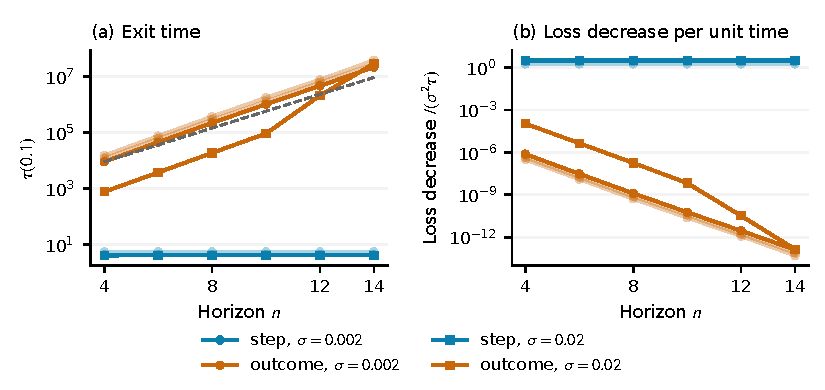
\includegraphics[width=\linewidth]{figures/regime_both.pdf}
\caption{\textbf{Outcome exit time grows at least as fast as $\mixrate^{-n}$; step exit time stays constant.}
Runs satisfy the assumptions of \cref{thm:outcome-end}, with a zero initial readout. Counting, $K=2$, $\mixrate=0.5$,
$\initscale=0.002$ and $0.02$, exact full-batch loss, no ReLU unit switching. (a)~Training time to leave the ball.
(b)~Loss decrease per unit time, in units of $\initscale^2$. Faint lines: two more draws of $\tilde\theta$.}
\label{fig:regime}
\end{figure}

\newpage
\section{Experiments test the mechanism}
\label{sec:validation}

We first test the bounds inside their assumptions (\cref{app:exp-regime}).
We then test the mechanism with LayerNorm, deeper models and LoRA.
Besides counting, we use Boolean-8 and a reversible register machine.
\Cref{tab:main} summarizes held-out accuracy; \cref{app:experiments} gives the protocols.

\begin{table}[t]
\centering\small
\fitwidth{\begin{tabular}{@{}llccccc@{}}
\toprule
Task & Model & $n$ & $\mixrate$ & outcome & step & chance\\
\midrule
count mod $2$ & two-block & $16$ & $0.50$ & $49$--$52$ & $100$ ($9$ of $10$ seeds) & $50$\\
count mod $3$ & two-block & $16$ & $0.66$ & $30$--$50$ & $100$ & $33$\\
first occurrence (control) & two-block & $8$--$24$ & -- & $71$--$100$ & $80$--$99$ & --\\
Boolean-8 & GPT-2L & $8$ & $0.82$ & $7.7$ & $82$ & $6.25$\\
register machine & GPT-2L & $16$ & $0.95$ & $6.3$ & $99.9$ & $5.9$\\
Boolean-8 & Qwen2.5-0.5B LoRA & $8$ & $0.82$ & $11.1$ & $98.3$ & $6.25$\\
\midrule
BBH, $3$ objects & Qwen2.5-0.5B LoRA & $3$ & $0$ & $35.2$ & $98.4$--$100$ & $33$\\
BBH, $5$ objects & Qwen2.5-0.5B LoRA & $5$ & $0.50$ & $80.0$--$94.4$ & $46$--$100$ & $20$\\
BBH, $7$ objects & Qwen2.5-0.5B LoRA & $7$ & $0.67$ & $15.2$--$24.4$ & $96.4$--$100$ & $14$\\
\bottomrule
\end{tabular}}
\caption{\textbf{Answers alone fail where the answer has no low-degree part; steps succeed.}
Accuracy (\%) on held-out prompts, ranges over seeds; the BIG-Bench Hard rows test on the $750$ real
items. First occurrence keeps a degree-$1$ part at every $n$, and outcome learns it. For count mod $2$ at $n=16$,
step accuracy is after $16$k updates and outcome after $32$k, twice the step budget. Protocols and per-seed results are
in \cref{app:experiments}.}
\label{tab:main}
\end{table}

\subsection{Spectra and gradients at initialization}

\paragraph{Predictions 1 and 2: degree mismatch.}
At initialization, the two-block Transformer's Jacobian puts $99.6\%$ of its mass at
degree $0$ (\cref{fig:overlap}). The targets put most of their mass at high degree.
For Boolean-8 and the register machine, $98.9\%$ and $99.9\%$ of answer variance is at
degrees $\ge2$.
The pattern also appears in Qwen2.5-0.5B.
On three-object BIG-Bench Hard, only $0.022\%$ of the LoRA Jacobian energy is at degree $3$,
the answer's only degree (\cref{app:exp-spectra}).

\paragraph{Prediction 3: gradient decay.}
Exact sums over counting prompts give answer-dependent gradient decay of $0.48$--$0.51$
per letter, close to $\mixrate=0.5$.
The step gradient grows $2.4$-fold from $n=2$ to $10$
(\cref{fig:credit,tab:spectrum}).

\subsection{Training}

\begin{samepage}
\paragraph{Prediction 4: plateau and escape.}
Across $120$ counting runs at $n=6$--$16$, outcome training solves none and step training
solves $60$ (\cref{app:exp-plateau}).
Step learning is still slow and seed-dependent: rule credit starts at order $\initscale^6$.
At $\initscale=0.1$, every tested step seed solves, while outcome training stays at chance
at $n=16$.
During the outcome plateau, at most $2\times10^{-6}$ of the Jacobian energy lies above
degree $1$ in the run shown in \cref{tab:main-evidence}.
\par
\end{samepage}

\begin{table}[!b]
\centering\small
\begin{tabular}{@{}lcc@{}}
\toprule
outcome updates & share above degree $1$ & accuracy\\
\midrule
initialization & $2.4\mathrm{e}{-6}$ & --\\
$1{,}000$ & $1.1\mathrm{e}{-8}$ & $52\%$\\
$3{,}000$ & $1.1\mathrm{e}{-8}$ & $48\%$\\
$6{,}000$ & $2.0\mathrm{e}{-6}$ & $48\%$\\
$8{,}000$ (escaping) & $0.155$ & $55\%$\\
\bottomrule
\end{tabular}
\caption{\textbf{The outcome plateau stays low-degree.} Counting, $K=2$, $n=8$: share of the
outcome model's Jacobian energy above degree $1$ during training, and answer accuracy.}
\label{tab:main-evidence}
\end{table}

\subsection{Transfer to a pretrained model}

\paragraph{Prediction 5: real object tracking.}
We train rank-8 LoRA on generated BIG-Bench Hard tracking\_shuffled\_objects items
\citep{suzgun2022challenging}. We test on all $750$ real benchmark items.
At three objects, $\mixrate=0$ and the answer is pure top degree.
Outcome training stays at the majority-option rate; step training reaches $98$--$100\%$.
The five- and seven-object results are less uniform (\cref{tab:main}).
\Cref{sec:discussion} discusses what the low-degree signal can predict.

\section{Related work}
\label{sec:related}

\paragraph{Intermediate supervision.}
Scratchpads and process supervision
\citep{nye2021scratchpads,uesato2022solving,wei2022cot,lightman2023verify}
have been studied through task decomposition \citep{wies2023subtask}, locality
\citep{prystawski2023think,abbe2024globality} and expressivity
\citep{feng2023towards,merrill2024expressive}.
Outcome supervision need not be statistically harder \citep{jia2025verify}.
Chain supervision can have better sample complexity
\citep{hanneke2026samplecomplexityautoregressivereasoning}.
We study how a fixed network distributes gradient credit at initialization.

\paragraph{Composed targets and gradient signal.}
\citet{shalevshwartz2017failures} show exponentially weak target-dependent gradients
across families of composed targets.
We decompose the credit of one fixed target and a concrete Transformer by degree.
Staircase and leap analyses
\citep{abbe2021staircase,abbe2022mergedstaircase,abbe2023sgd}
study when SGD can learn high-degree targets.
For our counting targets at $\mixrate>0$, all degrees are present.
Their size, rather than their absence, limits credit.
Step targets are known to help with parity and group tracking
\citep{wen2024sparse,liu2023automata}. \citet{panigrahi2025progressive} show that intermediate teacher
checkpoints supply low-degree signal that the final teacher lacks, reducing the sample complexity of
sparse parity; intermediate states play the same role here, and we analyze optimization rather than
sample complexity.

\paragraph{Hardness for a single target.}
\citet{abbe2025parities} prove that noisy gradient descent on a two-layer network stays at
chance on high-degree parities for $\exp(o(d))$ steps under Gaussian initialization, while
Rademacher initialization learns them; their argument is limited to the correlation loss.
\Cref{thm:outcome-end} concerns one fixed target for a Transformer under cross-entropy and exact
gradient descent. Its time $\mixrate^{-n}$ comes from the contraction of the target, resolved degree by degree.

\paragraph{Chain of thought for parity.}
\citet{kim2024parity} prove that a one-layer Transformer with position-only attention and a fixed
nonlinearity learns $k$-parity in one teacher-forced gradient step, and that gradient methods
without intermediate supervision fail for a parity drawn at random from a class. Their signal is
the degree-$2$ local interaction that our rule credit measures. Our negative result concerns one
fixed target; our positive result holds once the loss falls below an explicit threshold, for a
Transformer that learns its computation.

\paragraph{Permutation learning.}
\citet{wang2025compositional} study compositions of hidden permutations.
They give a statistical-query lower bound and a curriculum result at depth $O(\log k)$
\citep{sanford2024transformers}.
Our target is fixed, and displayed states permit constant-depth executors.
Their convergence result uses simplified dynamics; ours is local (\cref{thm:basin}).
\citet{li2025noise} decompose the target using Efron--Stein; we also decompose the Jacobian.
In single-layer Transformers on Markov data, the unigram solution can be stationary
\citep{makkuva2025attention,makkuva2024local}.
Here, outcome credit is small but need not vanish.

\section{Discussion}
\label{sec:discussion}

\paragraph{When do steps help?}
Low-degree answer variance estimates how much signal a fresh network can use; it is a diagnostic.
Five-object BIG-Bench Hard has only $1.56\%$ at degrees $0$--$1$, yet outcome training learns.
Its degree-$1$ signal is damped by $\mixrate^4=1/16$, rather than removed.
Low-degree share orders learning in the fixed-swap pilots, but not across swap counts (\cref{tab:bbh-pilot}).

\paragraph{Initialization scale.}
The target spectrum does not depend on initialization; the Jacobian spectrum does.
Larger initialization can improve step training, as the measured runs show.
The small-initialization bounds do not rule out outcome learning at other scales.

\paragraph{Parity.}
Counting modulo $2$ with match probability $1/2$ has $\mixrate=0$: only degree $n$ remains, giving
leap $n$ \citep{abbe2023sgd}. \Cref{rem:lambda-zero} handles this case.

\paragraph{Limitations.}
The assumptions in \cref{sec:intro} restrict the credit theorems.
AdamW runs allow ReLU switching and test the mechanism outside that regime
(\cref{rem:two-block-bias}).
The missing training result is entry into the step basin.
We have not tested large-scale training.

\paragraph{Conclusion.}
Interaction degree links the target to the gradient features available for learning,
explaining weak outcome credit and the signal retained by step targets.
Proving that step training reaches the basin is the remaining step.
